\chapter{Perspectiva de Solução} \label{chap:solução}

O reconhecimento facial em imagens sofreu uma evolução notável nos últimos 20 anos, tal como documentado no capítulo \ref{chap:reco} deste relatório. 

Em cenários cooperativos com condições de captura de imagens controladas, nomeadamente ao nível da pose, iluminação e expressões faciais, considera-se mesmo que o problema de verificação 1:1 se encontra resolvido, uma vez que as taxas de reconhecimento atingidas são satisfatórias para a grande maioria das aplicações \citep{Li2011}. Existem também várias aplicações em situações reais com um bom nível de satisfação por parte dos seus utilizadores, como é o caso do sistema de fronteira automático dos aeroportos portugueses, ou o controlo de entradas nas cerimónias inaugurais dos jogos olímpicos de Pequim. Em condições favoráveis, é então possível considerar que os sistemas de reconhecimento facial automático atuais conseguem mesmo ultrapassar a capacidade de reconhecimento humana, uma vez que conseguem identificar com precisão um maior número de faces do que aquelas que um humano consegue.

Contudo, o problema de reconhecimento facial automático ainda se encontra longe de ser um problema totalmente resolvido. Em cenários onde é registada uma grande variação ao nível da pose, iluminação ou outros fatores identificados na secção \ref{desafios} deste relatório, a identificação das entidades capturadas é ainda uma tarefa desafiante  \citep{Li2011}. Para além disso, a performance e satisfação obtida por parte dos utilizadores dos sistemas atuais demonstra uma grande variação tendo em conta as situações onde estes sistemas são utilizados. 

Finalmente, a crescente ubiquidade tecnológica e poder computacional presente nos diversos dispositivos utilizados no nosso dia a dia, aumenta o leque de aplicações possíveis do reconhecimento facial automático, apresentando novos desafios às soluções de atualmente existentes.

Assim sendo, torna-se pertinente a continuação da investigação na área do reconhecimento facial em imagens. Para além disso, o elevado valor comercial das soluções existentes e consequente falta soluções abertas permite aos resultados alcançar uma grande visibilidade dos resultados obtidos.

Ao nível da abstração de imagens, estudos efetuados demonstraram que aplicação destes filtros na recuperação de informação multimédia, nomeadamente no âmbito da da ilustração automática de texto têm a potencialidade de melhorar a informação retornada, assim como reduzir significativamente as necessidades de processamento e armazenamento \citep{Coelho2012}. 

Tendo a importância da investigação na área do reconhecimento facial, e uma vez que não existem estudos relativos à utilização de filtros de abstração no processo de reconhecimento facial, torna-se pertinente o estudo do seu impacto.

A hipótese levantada no âmbito desta dissertação é então que o uso de a abstração em imagens que vão ser ser alvo de reconhecimento facial pode melhorar a qualidade do reconhecimento.

\section{Objetivos} \label{sec:objetivosperpectiva}
O principal objetivo deste projeto visa o estudo do impacto de filtros de abstração visual de informação no processo de reconhecimento facial automático em imagens. Para isso, destacam-se o seguinte conjunto de objetivos parciais:

\begin{enumerate}
\item Desenvolvimento de um sistema de reconhecimento facial de personalidades;
\item Integração da abstração de imagens no sistema desenvolvido;
\item Avaliação dos resultados da abstração de imagens no processo de reconhecimento facial;
\end{enumerate}

Da avaliação efetuada, para além da publicação desta dissertação, espera-se ainda a publicação de um artigo científico onde sejam descritos os resultados obtidos.

\section{Implementação} \label{sec:implementacao}

Uma vez que não se pretende no âmbito desta dissertação efetuar investigação ao nível dos algoritmos de reconhecimento facial, mas sim ao nível do impacto do uso de imagens abstraídas nesse sistemas, a implementação desses algoritmos terá por base a utilização de soluções abertas de reconhecimento facial, nomeadamente a biblioteca \textit{Open CV (Open Source Computer Vision)}.

Ao nível dos filtros de abstração o estudo será efetuado utilizado o filtro \textit{Anisotropic Kuwahara}.
Este filtro foi utilizado anteriormente, e com resultados positivos, em abstração de imagens para a recuperação de informação multimédia, pelo que se considera adequada a sua utilização no âmbito deste projeto.

Por último, ao nível da coleção de dados a analisar, e uma vez que este projeto se encontra a ser desenvolvido em parceria com o laboratório da Sapo da FEUP, temos em vista analisar a coleção de imagens Sapo Fama, a qual agrega uma base de dados de imagens de personalidades famosas nacionais e internacionais.
	
\subsection{OpenCV - Face Recognizer}
O \textit{OpenCV} é uma biblioteca de código aberto nas áreas de visão por computador e \textit{machine learning}, onde se encontra disponível a implementação de mais de 2500 algoritmos. Esta biblioteca possui uma comunidade de mais de 47 mil pessoas, já registou mais de 5 milhões de downloads e é utilizada globalmente por empresas como a Google, Yahoo, Microsoft, Intel, IBM, Sony, Honda, Toyota \cite{Team}. 

Ao nível do reconhecimento facial, esta biblioteca disponibiliza um módulo denominado \textit{Face Recognizer}, onde se encontra implementados os algoritmos \textit{Eigenfaces}, \textit{Fisherfaces} e \textit{Local Binary Patterns Histograms}.

Tendo em conta a ampla utilização da biblioteca OpenCV e a sua constante atualização pela sua comunidade, assim como as facilidades providenciadas pelo módulo de reconhecimento facial, esta foi considerada a biblioteca ideal para utilizar como base de implementação do sistema de reconhecimento facial a criar. De seguida encontram-se brevemente descritos os três algoritmos implementados no módulo \textit{Face Recognizer:}

\subsubsection{Eigenfaces}
lorem ipsum

\subsubsection{Fisherfaces}
lorem ipsum

\subsubsection{Local Binary Patterns Histograms}
lorem ipsum

No âmbito desta dissertação será utilizado o algoritmo ?...todos?

\subsection{	Filtro \textit{Anisotropic Kuwahara}}
\begin{figure}[h]
  \begin{center}
    \leavevmode
    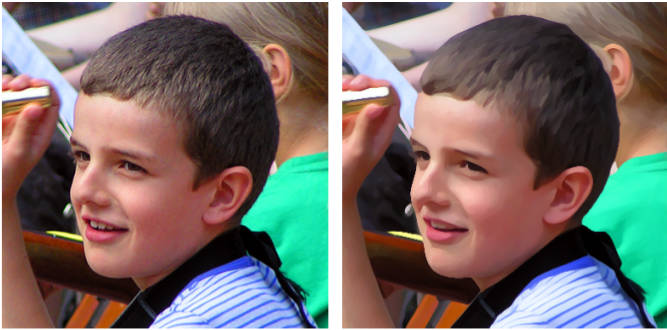
\includegraphics[width=0.7\textwidth]{filterskid}
    \caption{Comparação entre imagem não abstraída (esquerda) e imagem abstraída (direita).}	
    \label{fig:filterskid}
  \end{center}
\end{figure}

Ao nível dos filtros de abstração o estudo será efectuado utilizado o filtro Anisotropic Kuwahara (FAK).

Este filtro consiste numa generalização do filtro Kuwahara que remove alguns artefactos originados na aplicação do filtro original através da adaptação da forma, escala e orientação do filtro à estrutura local das características da imagem \cite{Kyprianidis2009}. Desta forma é produzido um efeito de abstração tipo pintura, onde é removida informação não essencial em zonas de elevado contraste, enquanto são preservados os limites representados nas zonas de menor contraste, tal como demonstrado na figura \ref{fig:filterskid}. As imagens ficam assim com a clareza de uma ilustração, mas preservam a informação direcional tal como nas pinturas a óleo clássicas. Por outro lado, este filtro tira partido da placa gráfica para a realização da abstração das imagens, tornando-se assim particularmente indicado para o processamento de um elevado número de fotografias.

O filtro em questão foi também utilizado anteriormente, e com resultados positivos, em abstração de imagens para a recuperação de informação multimédia. 

Tendo em conta os fatores apresentados consideramos que este filtro é o mais adequado para a utilização no âmbito deste projeto.

\subsection{Coleções de dados}
Ao nível das coleções de dados a analisar serão utilizadas duas coleções de dados Sapo Fama e \textit{Labeled Faces in the Wild}.

\subsubsection{Sapo Fama}
A coleção Sapo Fama será obtida no âmbito da integração desta dissertação no laboratório da Sapo da Universidade do Porto. Este galeria multimédia agrega uma coleção de imagens utilizadas na plataforma online de notícias sobre personalidades públicas da Sapo e respetivas descrições textuais. As imagens contidas nesta coleção representam uma oportunidade única de avaliação do sistema desenvolvido numa biblioteca de imagens real e com elevado valor comercial. Na figura \ref{SapoFama} encontram-se representados alguns exemplos das imagens contidas nesta coleção. 

\begin{figure}[t]
  \begin{center}
    \leavevmode
    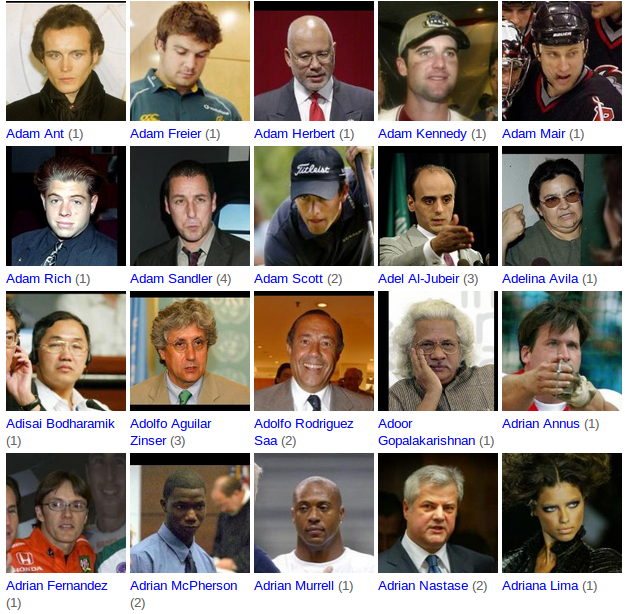
\includegraphics[width=1\textwidth]{lfw}
    \caption{Exemplos de imagens e respetivas anotações incluídas na biblioteca LFW}	
    \label{fig:lfwimagem}
  \end{center}
\end{figure}

\subsubsection{\textit{Labeled Faces in the Wild}}
A coleção \textit{Labeled Faces in the Wild (LFW)} é uma base de dados fotográfica desenhada especificamente para o estudo do problema de reconhecimento facial, particularmente em situações onde as condições de captura das imagens não possuem restrições. Esta coleção possuí 13233 imagens, de 5749 pessoas diferentes, sendo que dessas pessoas 1680 possuem mais do que uma imagem na galeria. O uso desta galeria no âmbito desta dissertação permitirá efetuar uma análise dos resultados obtidos num conjunto de dados standard e já previamente analisado por outros investigadores, assim como agilizar os testes dos sistemas desenvolvidos uma vez que a coleção já se encontra preparada especificamente para o estudo do desempenho de sistemas de reconhecimento facial automático. Na figura \ref{lbw} encontram-se representados alguns exemplos das imagens contidas nesta coleção.

\subsection{Avaliação Performance}
(explicar três sub-casos?)
A performance em sistemas de reconhecimento facial pode ser avaliada em taxa de deteção e identificação e taxa de falso-alarme. Um sistema de reconhecimento facial ideal teria uma taxa de deteção e identificação de 1.0 e uma taxa de falso-alame de 0.0.
//explicar taxas
//exemplo ROC 
\textit{Receiver Operating Characteristic (ROC)}



\subsection{Resultados Esperados}
Tendo em conta os resultados anteriormente observados no recurso à utilização de filtros de abstração para a ilustração automática de texto e o estado da arte da área de reconhecimento facial automático em imagens, o principal resultado esperado é que o uso de abstração de imagens melhore a qualidade do reconhecimento facial automático. No entanto, tendo em conta a complexidade do problema de reconhecimento facial automático, é também esperada alguma variação na performance verificada nos vários casos de teste.

Adicionalmente, espera-se que o uso da abstração de imagens leve a uma redução das necessidades de processamento e armazenamento do sistema desenvolvido.

\subsection{Plano de Trabalho}

\begin{figure}[t]
  \begin{center}
    \leavevmode
    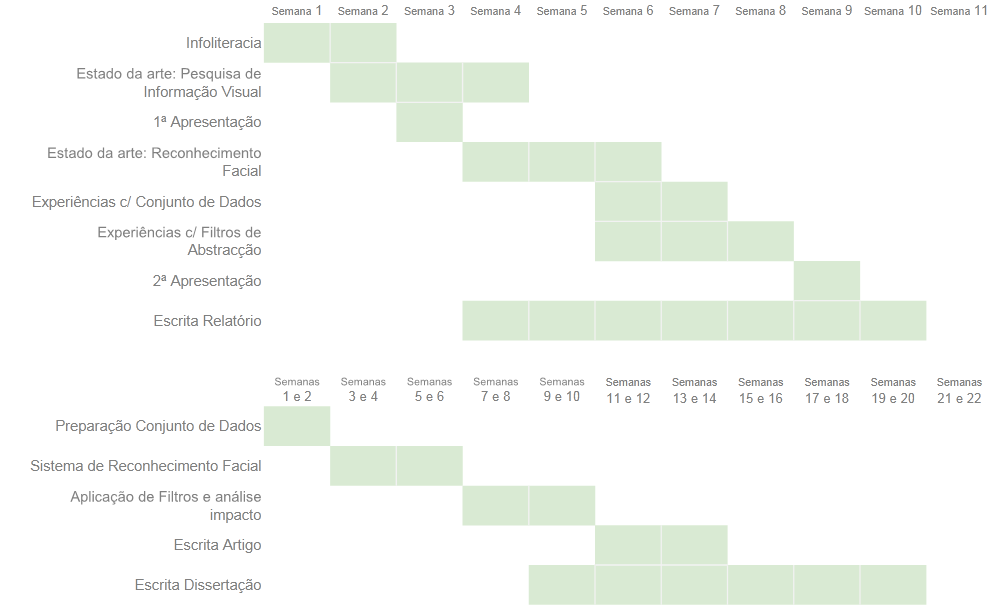
\includegraphics[width=0.9\textwidth]{GantSemSemanas}
    \caption{Plano de Trabalho 1º e 2º Semestres}	
    \label{fig:planotrabalho}
  \end{center}
\end{figure}

//Novo gant só com 2º semestre?

%Adicionalmente propõe-se também o desenvolvimento de um sistema de reconhecimento facial de personalidades que integre a abstração de imagens no processo de reconhecimento facial. Este sistema deverá ser capaz de detetar as faces presentes numa imagem e apresentar uma lista de possíveis entidades nela contidas.
